
%......................................
\subsubsection{The Stenberg macro-element} 

This macro-element is introduced in Stenberg (1984) \cite{sten84}. 

\begin{flushright} {\tiny {\color{gray} (tikz\_stenberg.tex)}} \end{flushright}
%~~~~~~~~~~~~~~~~~~~~~~~~~~~~~~~~~~~~~~~~~~~~~~~~~~~~~~~~~~~~~~~~~~~~~~~~~~~~~~~~~~~~~~~~~~~~~~~~~~

\begin{center}
\begin{tikzpicture}
%\draw[fill=gray!23,gray!23](0,0) rectangle (5,5);
%\draw[step=0.5cm,gray,very thin] (0,0) grid (6,4); %background grid
\draw[thick] (1,1) -- (5,1) -- (5,3) -- (1,3) -- cycle;  
\draw[thick] (3,1) -- (4,2) -- (3,3) -- (2,2) -- cycle;  
\draw[thick] (1,2) -- (2,2);  
\draw[thick] (4,2) -- (5,2);  

\draw[black,fill=teal] (1,1) circle (2pt);
\draw[black,fill=teal] (3,1) circle (2pt);
\draw[black,fill=teal] (5,1) circle (2pt);
\draw[black,fill=teal] (1,2) circle (2pt);
\draw[black,fill=teal] (2,2) circle (2pt);
\draw[black,fill=teal] (4,2) circle (2pt);
\draw[black,fill=teal] (5,2) circle (2pt);
\draw[black,fill=teal] (1,3) circle (2pt);
\draw[black,fill=teal] (3,3) circle (2pt);
\draw[black,fill=teal] (5,3) circle (2pt);

\draw[violet] (1.75,1.5) circle (4pt);
\draw[violet] (1.75,2.5) circle (4pt);
\draw[violet] (4.25,1.5) circle (4pt);
\draw[violet] (4.25,2.5) circle (4pt);
\draw[violet] (3,2) circle (4pt);

\draw[black,fill=teal] (3,0.25)   circle (2pt);
\node[] at (3.4,0.2) {$\vec\upnu$};

\draw[violet] (4.1,0.2) circle (4pt); 
\node[] at (4.4,0.2) {$p$};

\end{tikzpicture}
\end{center}




Gresho \& Sani \cite{grsa} state: "For fans of $Q_1\times Q_0$ who want 
guaranteed optimal convergence of both $u$ and $p$ (with however larger error 
constants caused by the distorted shapes?), one way to assure this is
to discretise via the macro elements above, each composed of five $Q_1\times Q_0$
quadrilaterals. Such checkerboard-killer meshes have been employed in practice
by (at least) Bath\'e \cite{chba93}. Both the macro-element and the proof are
due to Stenberg \cite{sten84}."

Chapelle \& Bathe \cite{chba93}: "the numerical inf-sup test is passed for this mesh and in fact,
this behavior was proven analytically (see Brezzi \& Fortin \cite{brfo}, see 
also Le Tallec \& Ruas \cite{leru86}).

\begin{center}
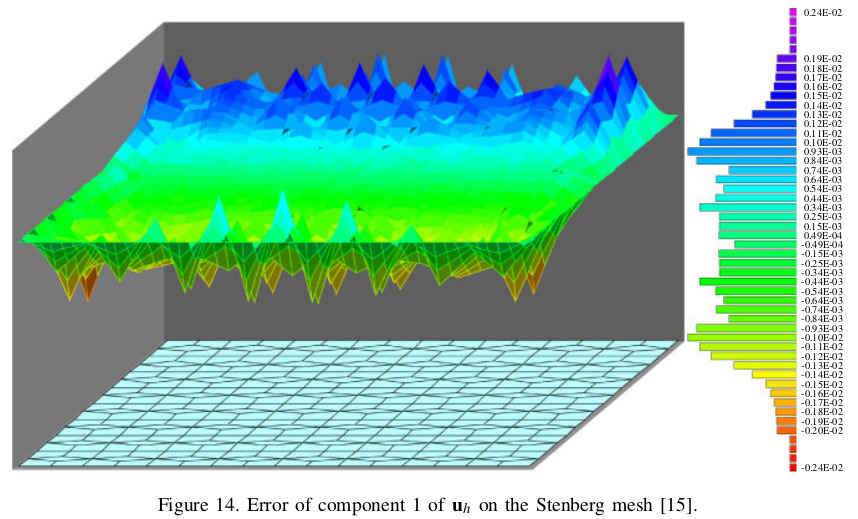
\includegraphics[width=5cm]{images/meshtopos/qizh07}\\
{\captionfont Taken from Qin \& Zhang (2007) \cite{qizh07}.}
\end{center}

Implemented in \stone~78.

\Literature: Fig 3.12 of Elman \etal book \cite{elsw}.

%......................................
\subsubsection{The Le Tallec macro-element} 

This macro-element is introduced in Le Tallec (1981) \cite{leta81}.

\begin{flushright} {\tiny {\color{gray} (tikz\_letallec.tex)}} \end{flushright}
%~~~~~~~~~~~~~~~~~~~~~~~~~~~~~~~~~~~~~~~~~~~~~~~~~~~~~~~~~~~~~~~~~~~~~~~~~~~~~~~~~~~~~~~~~~~~~~~~~~

\begin{center}
\begin{tikzpicture}
%\draw[fill=gray!23,gray!23](0,0) rectangle (5,5);
%\draw[step=0.5cm,gray,very thin] (0,0) grid (6,6); %background grid
\draw[thick] (1,1) -- (5,1) -- (5,5) -- (1,5) -- cycle;  
\draw[thick] (2,2) -- (4,2) -- (4,4) -- (2,4) -- cycle;  

\draw[thick] (1,1) -- (2,2);  
\draw[thick] (5,1) -- (4,2);  
\draw[thick] (1,5) -- (2,4);  
\draw[thick] (5,5) -- (4,4);  
\draw[thick] (1,3) -- (5,3);  
\draw[thick] (3,1) -- (3,5);  

\draw[black,fill=teal] (1,1)   circle (2pt);
\draw[black,fill=teal] (3,1)   circle (2pt);
\draw[black,fill=teal] (5,1)   circle (2pt);

\draw[black,fill=teal] (2,2)   circle (2pt);
\draw[black,fill=teal] (4,2)   circle (2pt);

\draw[black,fill=teal] (1,3)   circle (2pt);
\draw[black,fill=teal] (3,3)   circle (2pt);
\draw[black,fill=teal] (5,3)   circle (2pt);

\draw[black,fill=teal] (2,4)   circle (2pt);
\draw[black,fill=teal] (4,4)   circle (2pt);

\draw[black,fill=teal] (1,5)   circle (2pt);
\draw[black,fill=teal] (3,5)   circle (2pt);
\draw[black,fill=teal] (5,5)   circle (2pt);

\draw[violet] (2.25,1.5) circle (4pt);
\draw[violet] (3.75,1.5) circle (4pt);

\draw[violet] (1.5,2.25) circle (4pt);
\draw[violet] (1.5,3.75) circle (4pt);
\draw[violet] (2.5,2.5) circle (4pt);
\draw[violet] (3.5,2.5) circle (4pt);
\draw[violet] (2.5,3.5) circle (4pt);
\draw[violet] (3.5,3.5) circle (4pt);
\draw[violet] (4.5,2.25) circle (4pt);
\draw[violet] (4.5,3.75) circle (4pt);
\draw[violet] (2.25,4.5) circle (4pt);
\draw[violet] (3.75,4.5) circle (4pt);

\draw[black,fill=teal] (3,0.25)   circle (2pt);
\node[] at (3.4,0.2) {$\vec\upnu$};

\draw[violet] (4.1,0.2) circle (4pt); 
\node[] at (4.4,0.2) {$p$};

\end{tikzpicture}\\
\end{center}




This macro-element has been proven stable in \cite{leta81,leru86}, i.e. it satisfies 
the stability condition (see Section~\ref{ss:pair}).
It is also mentioned in Qin \& Zhang (2007) \cite{qizh07}.

Implemented in \stone 78.

%..............................................
\subsubsection{The Qin \& Zhang macro-elements}

In their paper Qin \& Zhang (2007) \cite{qizh07} the authors mention the Stenberg and Le Tallec
macro-elements and also introduce three new ones:

\begin{flushright} {\tiny {\color{gray} (tikz\_qizh07a.tex)}} \end{flushright}
%~~~~~~~~~~~~~~~~~~~~~~~~~~~~~~~~~~~~~~~~~~~~~~~~~~~~~~~~~~~~~~~~~~~~~~~~~~~~~~~~~~~~~~~~~~~~~~~~~~

\begin{tikzpicture}
%\draw[fill=gray!23,gray!23](0,0) rectangle (5,5);
%\draw[step=0.5cm,gray,very thin] (0,0) grid (6,6); %background grid
\draw[thick] (1,1) -- (5,1) -- (5,5) -- (1,5) -- cycle;  
\draw[thick] (1.75,3) -- (3,1.75) -- (4.25,3) -- (3,4.25) -- cycle;  

\draw[thick] (1,1) -- (5,5) ;  
\draw[thick] (1,5) -- (5,1) ;  

\draw[thick] (3,1) -- (3,1.75) ;  
\draw[thick] (3,4.25) -- (3,5) ;  

\draw[thick] (1,3) -- (1.75,3) ;  
\draw[thick] (4.25,3) -- (5,3) ;  

\draw[black,fill=teal] (1,1)   circle (2pt);
\draw[black,fill=teal] (3,1)   circle (2pt);
\draw[black,fill=teal] (5,1)   circle (2pt);

\draw[black,fill=teal] (3,1.75)   circle (2pt);
\draw[black,fill=teal] (2.375,2.375)   circle (2pt);
\draw[black,fill=teal] (3.625,2.375)   circle (2pt);

\draw[black,fill=teal] (1,3)   circle (2pt);
\draw[black,fill=teal] (1.75,3)   circle (2pt);
\draw[black,fill=teal] (3,3)   circle (2pt);
\draw[black,fill=teal] (4.25,3)   circle (2pt);
\draw[black,fill=teal] (5,3)   circle (2pt);

\draw[black,fill=teal] (2.375,3.625)   circle (2pt);
\draw[black,fill=teal] (3.625,3.625)   circle (2pt);
\draw[black,fill=teal] (3,4.25)   circle (2pt);

\draw[black,fill=teal] (1,5)   circle (2pt);
\draw[black,fill=teal] (3,5)   circle (2pt);
\draw[black,fill=teal] (5,5)   circle (2pt);

\draw[violet] (2.25,1.5) circle (4pt);
\draw[violet] (3.75,1.5) circle (4pt);

\draw[violet] (1.5,2.25) circle (4pt);
\draw[violet] (3,2.375) circle (4pt);
\draw[violet] (4.5,2.25) circle (4pt);

\draw[violet] (2.375,3) circle (4pt);
\draw[violet] (3.625,3) circle (4pt);

\draw[violet] (3,3.625) circle (4pt);
\draw[violet] (1.5,3.75) circle (4pt);
\draw[violet] (4.5,3.75) circle (4pt);

\draw[violet] (2.25,4.5) circle (4pt);
\draw[violet] (3.75,4.5) circle (4pt);

\draw[black,fill=teal] (3,0.25)   circle (2pt);
\node[] at (3.4,0.2) {$\vec\upnu$};

\draw[violet] (4.1,0.2) circle (4pt); 
\node[] at (4.4,0.2) {$p$};
\end{tikzpicture}




They also indicate that although stable, these macro-elements are inferior 
to the above two. 

%..............................................
\subsubsection{New macro-elements ?}

\begin{center}
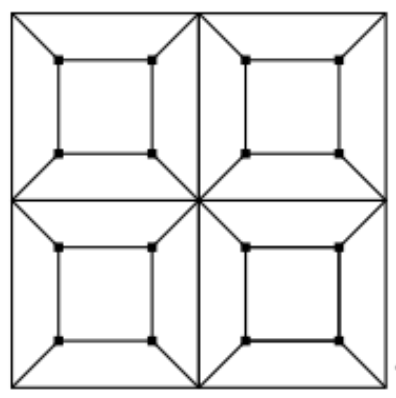
\includegraphics[width=4cm]{images/meshtopos/m21}
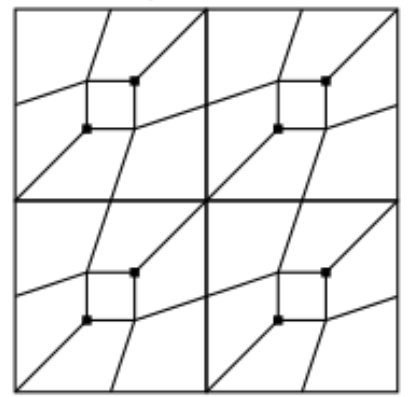
\includegraphics[width=4cm]{images/meshtopos/m22}
\end{center}

I came up with these, no idea whether these are stable/usable or better than the others.






 

